\section{Geometric Optics II}
We continue our discussion of geometric optics, where we reconcile our intuitive picture of light beams with the electromagnetic fields we have been studying.

\subsection{Review of Last Lecture}
We considered solutions:
\begin{equation}
    \psi(t, \v{x}) = \chi(\v{x})e^{-i\omega t}
\end{equation}
to the wave equation:
\begin{equation}
    \square \psi = 0
\end{equation}
therein, the spatial part $\chi(\v{x})$ satisfies the Helmholtz equation:
\begin{equation}
    \nabla^2 \chi + \frac{\omega^2}{c^2}\chi = 0
\end{equation}
which has approximate solutions:
\begin{equation}
    \chi(\v{x}) = A(\v{x})e^{iS(\v{x})}
\end{equation}
with $\abs{\nabla^2 A} \ll \abs{\nabla S}^2 A$. Then:
\begin{equation}
    \abs{\nabla S}^2 = \frac{\omega^2}{c^2}
\end{equation}
And:
\begin{equation}
    2\nabla S \cdot \nabla A + (\nabla^2 S)A = 0
\end{equation}
which is known as the geometric optics (or WKB) approximation. WE can then define the vector field $\v{k}(\v{x})$:
\begin{equation}
    \v{k}(\v{x}) = \nabla S \implies \abs{\v{k}}^2 = \frac{\omega^2}{c^2}
\end{equation}
where $\v{k}$ has constant length. 

\subsection{Properties of $\v{k}$ \& Light Rays}
The vector $\v{k}$ is orthogonal to the surface of constant phase at $\v{x}$. How do we see this? Suppose we consider a surface where $S(\v{x}) = \text{const.}$. 

\begin{center}
    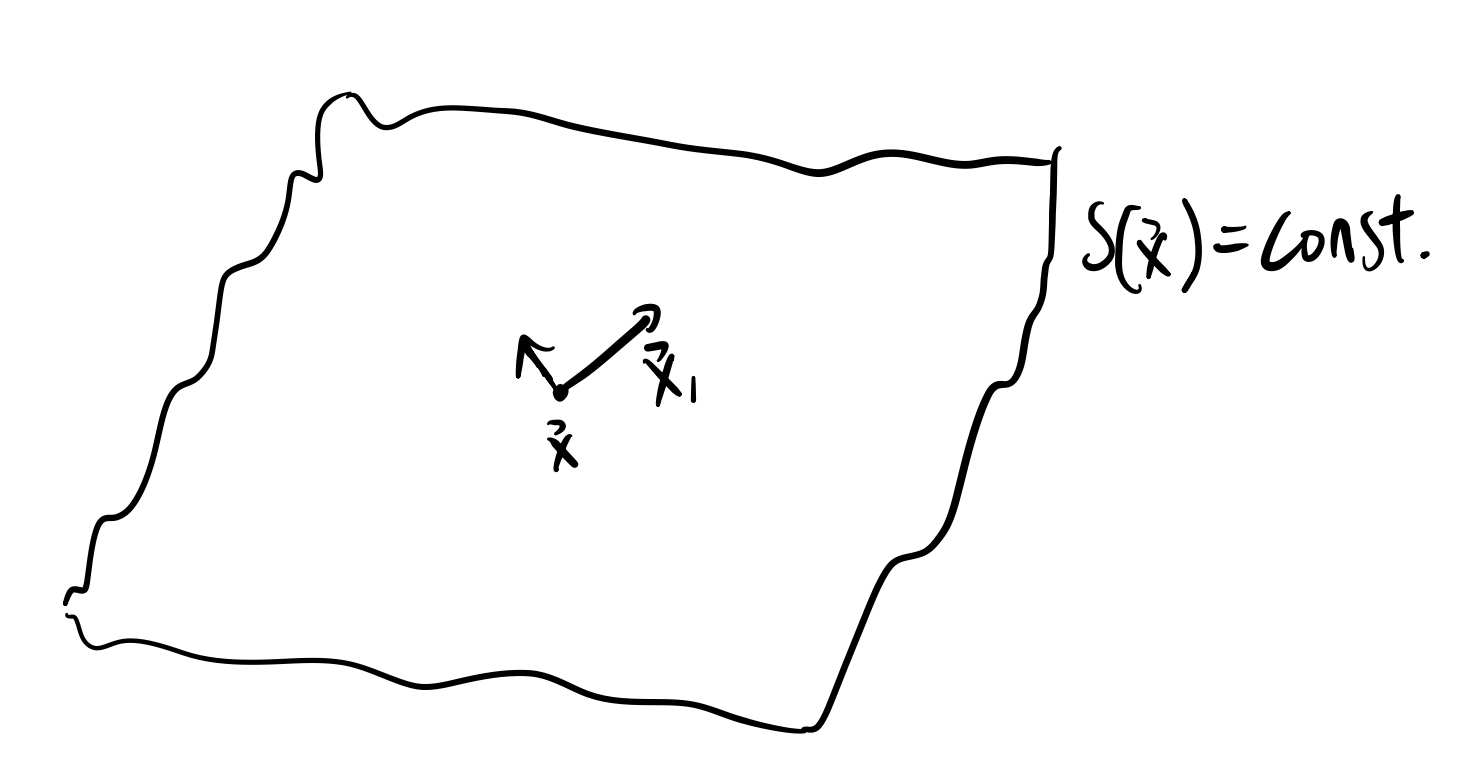
\includegraphics[scale=0.3]{Lectures/Images/lec17-constantphasesurface.png}
\end{center}

Now, we consider parameterizing the surface as:
\begin{equation}
    \v{x} + \beta \v{x}_1
\end{equation}
Therein, if we expand for $\beta \to 0$:
\begin{equation}
   0 = S(\v{x} + \beta\v{x}_1) = S(\v{x}) + \beta \v{x}_1 \cdot \nabla S(\v{x})
\end{equation}
So:
\begin{equation}
    \v{x}_1 \cdot \nabla S(\v{x}) = \v{x}_1 \cdot \v{k}(\v{x}) = 0
\end{equation}

Let us consider the integral curves $\v{x}(\alpha)$, defined by:
\begin{equation}
    \dod{\v{x}}{\alpha} = \v{k}(\v{x})
\end{equation}

\begin{center}
    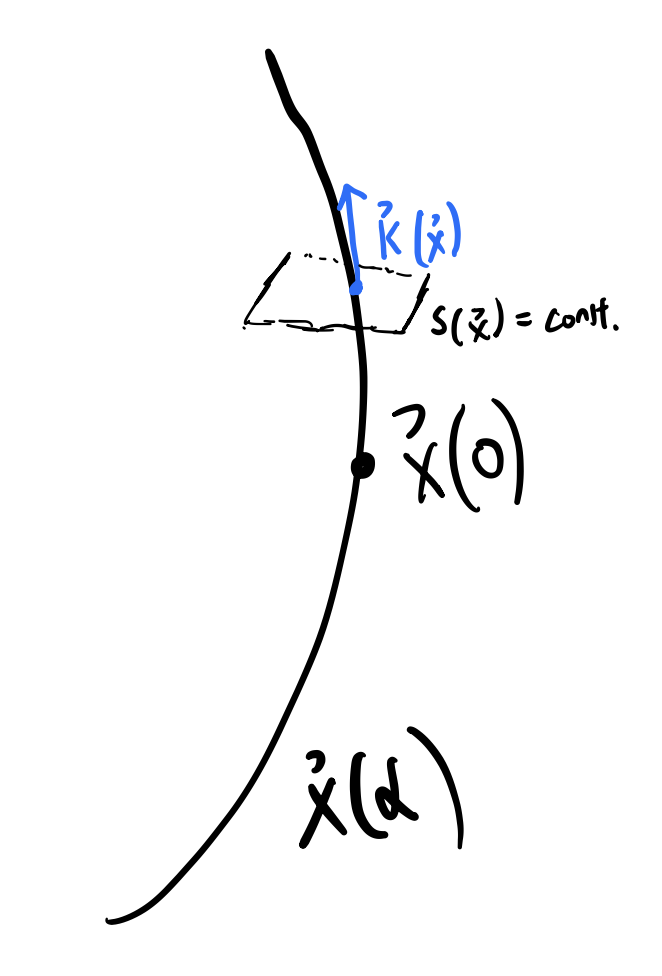
\includegraphics[scale=0.3]{Lectures/Images/lec17-ray.png}
\end{center}

Where $\v{k}(\v{x})$ is parallel to the curve at each point, and a single point $\v{x}(0)$ specifies which light ray we are on. We call these curves \emph{light rays}. What we notice is that these light rays are orthogonal to the surfaces of fixes $S$, for all $\v{x}$.

We drew the light ray as a curved line in the above sketch, but it turns out that all light rays are actually straight lines (so long as $n = 1$/the index of refraction is 1, which is the current setting). Let's prove this. We first look at:
\begin{equation}
    \left.(\v{k} \cdot \nabla)\v{k}\right|_i = k_j \p_j k_i = k_j \p_j \p_i S = k_j \p_i \p_j S = k_j \p_i k_j = \frac{1}{2}\p_i \abs{\v{k}}^2 = 0
\end{equation}
So in terms of integral curves:
\begin{equation}
    \left(\dod{\v{x}}{\alpha}\cdot\nabla\right)\dod{x_i}{\alpha} = 0
\end{equation}
This equation can be intepreted as (using the chain rule):
\begin{equation}
    \dod{}{\alpha} \left(\dod{x_i}{\alpha}\right) = 0
\end{equation}
This means that $\p_\alpha^2 x_i = 0$, and hence the light rays must be straight lines:
\begin{equation}
    \v{x}(\alpha) = \v{x}(0) + \v{v}(0)\alpha
\end{equation}

We can write the second equation in the geometric optics approximation as:
\begin{equation}
    2\v{k}(\v{x}) \cdot \nabla A + (\nabla \cdot \v{k})A = 0
\end{equation}
Let us rewrite this (using the product rule)
\begin{equation}
    \nabla \cdot (A^2\v{k}) = 0
\end{equation}
This has the intepretation as a continuity equation; suppose we have a continuous distribution of particles with number density $\rho_p \propto A^2$. If we consider some volume $V$, we can ask how many particles live in this volume; then:
\begin{equation}
    N_V = \int d^3\v{x} \rho_p
\end{equation}
The particles we take to be moving with speed $c$ in the direction of $\v{k}(\v{x})$. If the number of particles is conserved, we have a conservation equation:
\begin{equation}
    \dot{\rho_p} + \nabla \cdot \v{J}_p = 0
\end{equation}
now, $\rho_p \propto A^2(\v{x})$ which has no time dependence, so it must be that:
\begin{equation}
    \nabla \cdot \v{J}_p = 0
\end{equation}
where:
\begin{equation}
    \v{J}_p = A^2\v{k}.
\end{equation}
Recalling our wave equation solutions:
\begin{equation}
    \psi(t, \v{x}) = \chi(\v{x})e^{-i\omega t}
\end{equation}
where:
\begin{equation}
    \abs{\psi}^2 = \abs{\chi}^2 = \abs{A}^2
\end{equation}
we can see that $\abs{A}^2$ has the interpretation of a particle density.

\subsection{Fermat's Principle}
We can generalize to situations where the index of refraction is space-dependent, $n(\v{x})$. The wave equation looks like:
\begin{equation}
    \nabla^2 \psi - \frac{n^2(\v{x})}{c^2}\p_t^2 \psi = 0
\end{equation}
Without going through all of the algebra, we can see that the modifications to the geometric optics equations become:
\begin{equation}
    \abs{\nabla S}^2 = \frac{\omega^2}{c^2}n^2(\v{x})
\end{equation}
\begin{equation}
    2\nabla S \cdot \nabla A + (\nabla^2 S)A = 0 \quad (\text{no change})
\end{equation}
We can again define $\v{k} = \nabla S$, and we then obtain:
\begin{equation}
    (\v{k} \cdot \nabla)\v{k} = \frac{\omega^2}{c^2}n\nabla n
\end{equation}
So then:
\begin{equation}
    \dod[2]{\v{x}}{\alpha} = \frac{\omega^2}{c^2}n\nabla n
\end{equation}
and:
\begin{equation}
    \abs{\dod{\v{x}}{\alpha}} = \frac{\omega}{c}n(\v{x})
\end{equation}

We can consider an action:
\begin{equation}
    \mathcal{S} = \int d\lambda n(\v{x})\sqrt{\dod{\v{x}}{\lambda}\cdot\dod{\v{x}}{\lambda}}
\end{equation}
If we were to write the Euler-Lagrange equations for this action, we get precisely the equations for the integral curves. Why are we excited about this? This action has a very nice physical interpretation.

\begin{center}
    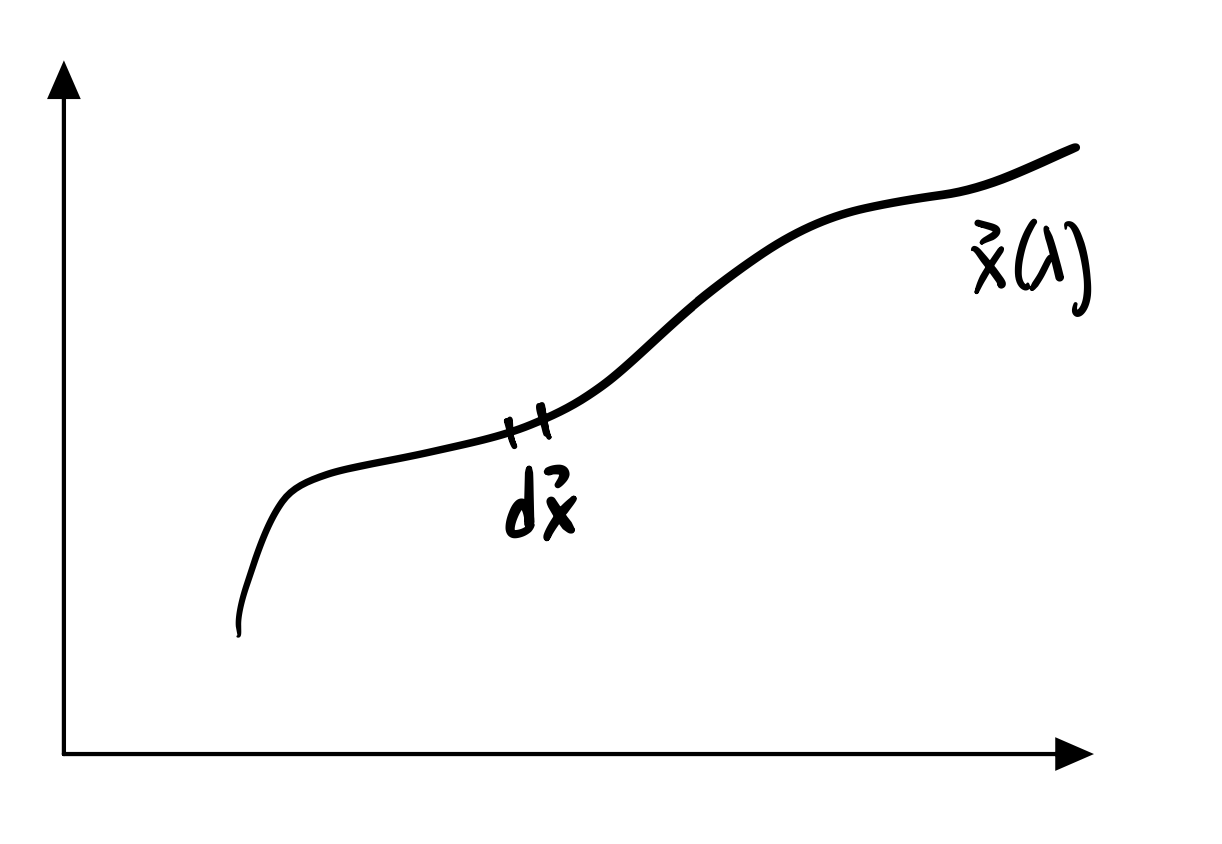
\includegraphics[scale=0.3]{Lectures/Images/lec17-trajectory.png}
\end{center}

If we have a particle propagating in space along this curve and it travels with speed $v = \frac{c}{n(\v{x})}$, $\mathcal{S}$ can be thought of as the elapsed time.

Suppose we consider the time it takes for a light ray to reach $A$ to $B$. The lower bound is precisely given by the extrema of the above action - this gives rise to \emph{Fermat's principle}; light rays are minima of the elapsed time functional, with the speed of propagation $\frac{c}{n(\v{x})}$.

If Kutasov had another problem set to give, he would give the following problem; consider the setup:

\begin{center}
    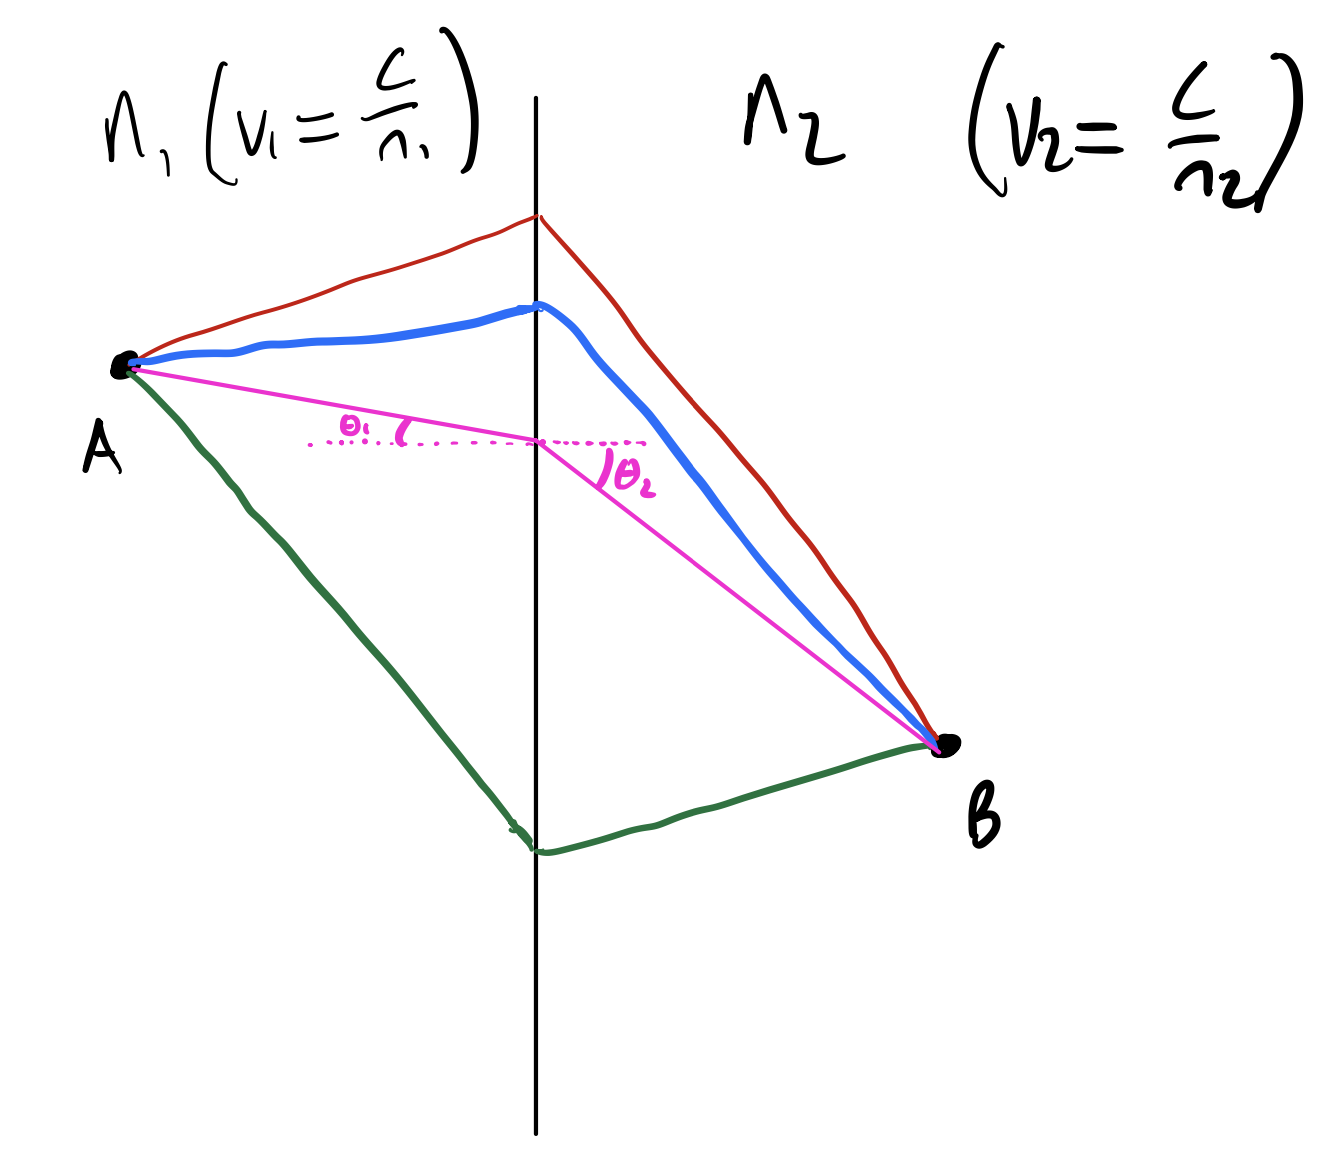
\includegraphics[scale=0.3]{Lectures/Images/lec17-snell.png}
\end{center}

For each possible trajectory we can compute the elapsed time. But the trajectory that minimizes the elapsed time is given by Snell's law:
\begin{equation}
    n_1\sin\theta_1 = n_2\sin\theta_2
\end{equation}

\subsection{Back to Electromagnetism}
We've been looking at the wave equation, but we should specify back to the theory we are actually studying. There, we have that the gauge potential satisfies the wave equation:
\begin{equation}
    \square A^\mu = 0
\end{equation}
and we work in the Lorentz gauge:
\begin{equation}
    \p_\mu A^\mu = 0
\end{equation}
Let us write the same kind of ansatz we did before with $\psi$:
\begin{equation}
    A_\mu(\v{x}, t) = F_\mu(\v{x})e^{-i\omega t}
\end{equation}
the gauge symmetry allows us to fix $A_0 = 0$ via an appropriate gauge transformation $A_\mu \to A_\mu + \p_\mu \alpha$. So, we only need worry about the vector potential, where the Lorentz gauge condition now tells us that:
\begin{equation}
    \nabla \cdot \v{A} = 0.
\end{equation}
We have:
\begin{equation}
    \v{A}(t, \v{x}) = C(\v{x})e^{iS(\v{x})}e^{-i\omega t}
\end{equation}
The geometric optics equation give us:
\begin{equation}
    \abs{\nabla S}^2 = \abs{\v{k}}^2 = \frac{\omega^2}{c^2}
\end{equation}
\begin{equation}\label{eq:geomopticsEM}
    2(\v{k} \cdot \nabla)\v{C} + (\nabla \cdot \v{k})\v{C} = 0
\end{equation}
and $\nabla \cdot \v{A} = 0$ tells us that:
\begin{equation}
    \v{k} \cdot \v{C} = 0
\end{equation}

Define light rays as integral curves of $\v{k}$ as before, where note $\v{C} \perp \v{k}$ for all $\v{x}$.

\begin{center}
    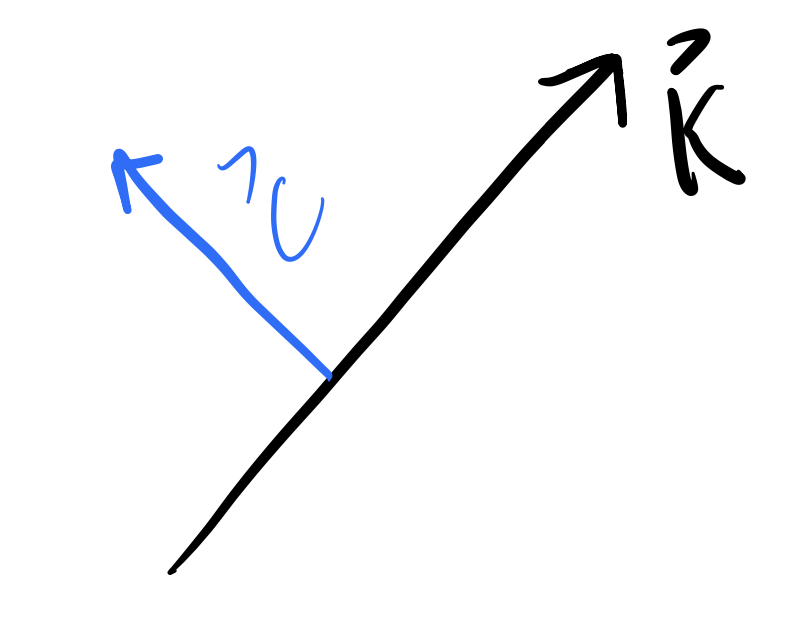
\includegraphics[scale=0.3]{Lectures/Images/lec17-Ck.png}
\end{center}

We could wonder whether $\v{C}$ could change direction in the plane orthogonal to $\v{k}$. But in fact the direction of $\v{C}$ does not change along a light ray. We study:
\begin{equation}
    \dod{}{\alpha}\v{C}(\v{x}(\alpha)) = \dpd{\v{C}}{x_i}\dpd{x_i}{\alpha} = (\v{k} \cdot \nabla)\v{C}
\end{equation}
Using Eq. \eqref{eq:geomopticsEM}:
\begin{equation}
    \dod{}{\alpha}\v{C} = -\frac{1}{2}(\nabla \cdot\v{k})\v{C}
\end{equation}
so $\p_\alpha \v{C}$ points in the direction of $\v{C}$, and it does so for all $\alpha$; we conclude that $\v{C}$ does not change direction as we move along the light ray (though it may change its magnitude).

Note that EM has an analogous conservation equation as we discussed in the general case:
\begin{equation}
    \nabla \cdot (\abs{\v{C}}^2\v{k}) = 0
\end{equation}

Finally - in a lab we measure $\v{E}, \v{B}$. Computing:
\begin{equation}
    \v{E} = -\dot{\v{A}} = -i\omega \v{C}(\v{x})e^{iS(\v{x})}e^{-i\omega t}
\end{equation}
\begin{equation}
    \v{B} = \nabla \times \v{A} = i\v{k} \times \v{C}e^{iS(\v{x})}e^{-i\omega t}
\end{equation}
hm - what about the terms where the derivative acts on the $\v{C}$? Yes, there is such a $\sim \nabla \times \v{C}$ term, but we may neglect it because all of this is done in an approximation where the amplitude varies much more slowly than the phase $\abs{\nabla^2 \v{C}}^2 \ll \abs{\nabla S}^2\abs{\v{C}}$, so we may drop this term.

So, we have a very familiar situation. The wave propagates in the $\v{k}$ direction. The electric field is in the $\v{C}$ direction orthogonal to $\v{k}$, and the magnetic field is $\sim \v{k} \times \v{C}$ so it is orthogonal to the other two. This is the usual statement of dealing with transverse EM waves. One can calculate the Poynting vector:
\begin{equation}
    \v{S} = \frac{1}{\mu_0}\Re(\v{E}) \times \Re(\v{B})
\end{equation}
where:
\begin{equation}
    \v{S} \propto \abs{\v{C}}^2\v{k}
\end{equation}
The story with Fermat's principle, Snell's Law works exactly the same here - we can introduce a nontrivial index of refraction $n(\v{x})$ exactly in the same way. Actual light rays are indeed described by the same Lagrangian, because all of the complication of looking at the gauge potential $A_\mu$ does not enter.